

%%%%%% General PETSc information %%%%%%%%%%

%%% What is PETSc



\begin{frame}[fragile]
\frametitle{PETSc Pyramid}
 \begin{block}{PETSc Structure} \vspace{0.3cm}
   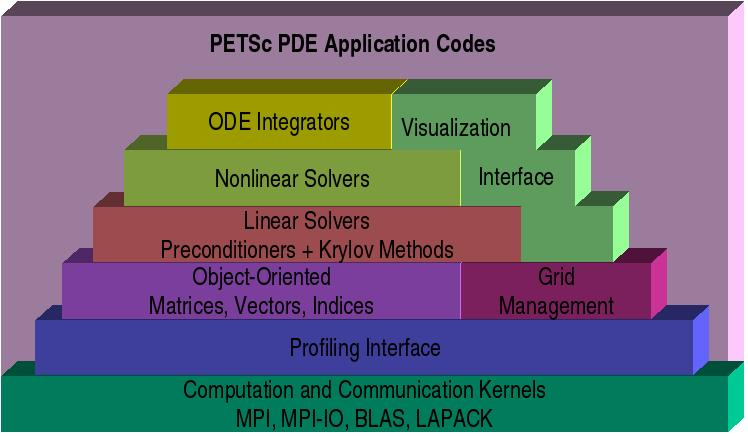
\includegraphics[width=1.0\textwidth]{PETScPyramid.jpg}
 \end{block}

\end{frame}

\begin{frame}[fragile]
\frametitle{Flow Control for a PETSc Application}

\begin{center}
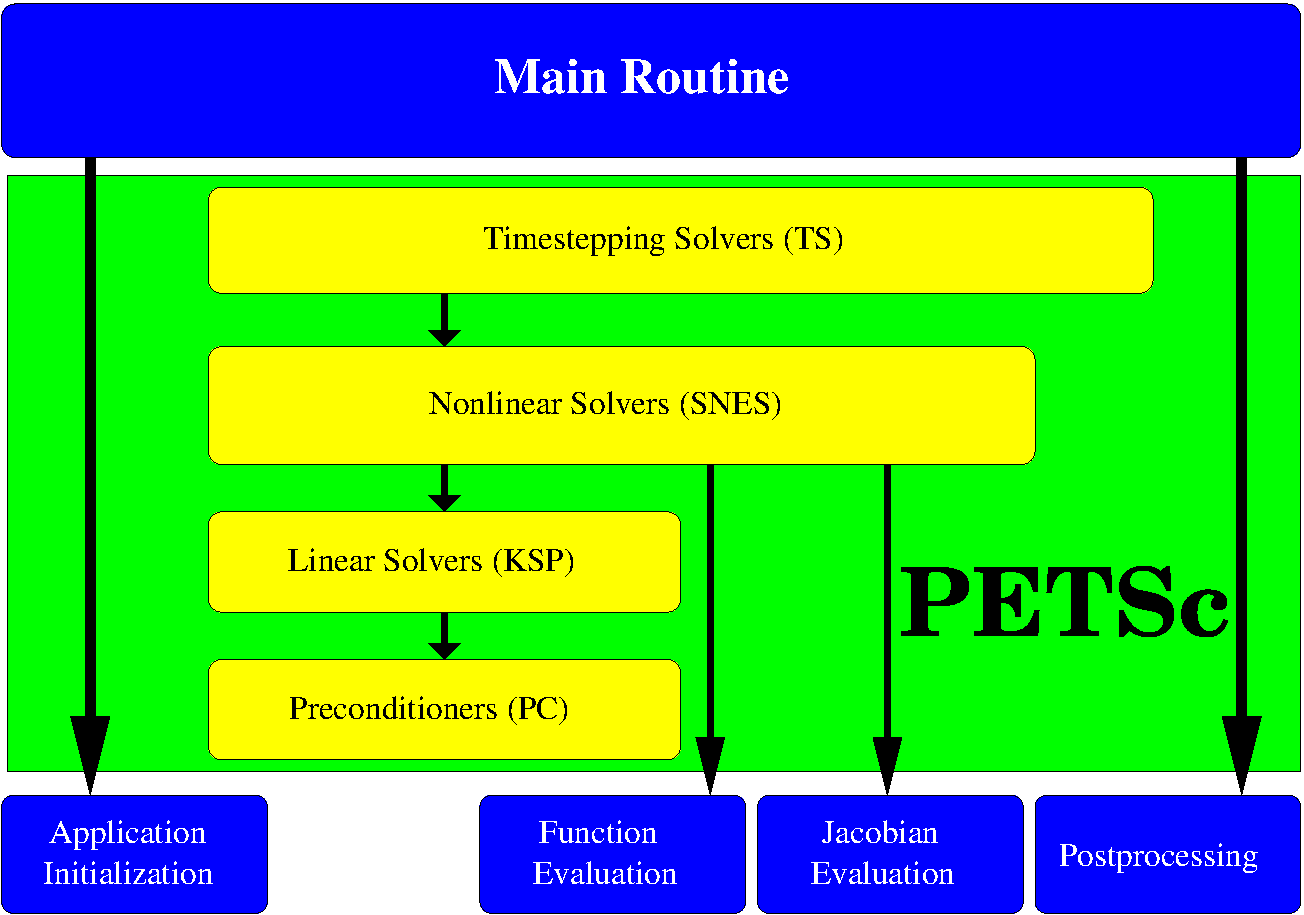
\includegraphics[width=4.0in]{figures/FlowControl}
\end{center}
\end{frame}



\section{PETSc Overview}
\begin{frame}{PETSc}
   \begin{center} \Large \textbf{Vectors and Matrices} \end{center}
\end{frame}



\begin{frame}[fragile]

\frametitle{The Role of PETSc}

\vspace*{\fill}
\begin{minipage}{\linewidth}
\begin{quote}
\Large You want to think about how you decompose your data
structures, how you think about them globally. [...] 

\medskip 

If you
were building a house, you'd start with a set of blueprints
that give you a picture of what the whole house looks
like. You wouldn’t start with a bunch of tiles and say.
``Well I'll put this tile down on the ground, and then I'll
find a tile to go next to it.''

\medskip

But all too many people try to
build their parallel programs by creating the smallest
possible tiles and then trying to have the structure of
their code emerge from the chaos of all these little
pieces. You have to have an organizing principle if
you're going to survive making your code parallel.

\end{quote}

\qquad --- Bill Gropp

\qquad --- http://www.rce-cast.com/Podcast/rce-28-mpich2.html
\end{minipage}
\vspace*{\fill}\vspace*{\fill}

\end{frame}





\begin{frame}[fragile]{PETSc Vectors}

 \begin{block}{Parallel Vector Layout}
   \begin{center}
     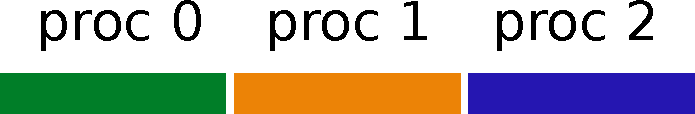
\includegraphics[width=0.75\textwidth]{figures/vectors} \\[2em]
   \end{center}
\begin{lstlisting}
  VecCreate(PETSC_COMM_WORLD, &x);
  VecSetSizes(x, PETSC_DECIDE, N);
  VecSetFromOptions(x);
\end{lstlisting}
  \vspace*{2.3cm}
 \end{block}

\end{frame}

\begin{frame}[fragile]{PETSc Vectors}

 \begin{block}{Vector Gather and Scatter}
   \begin{center}
     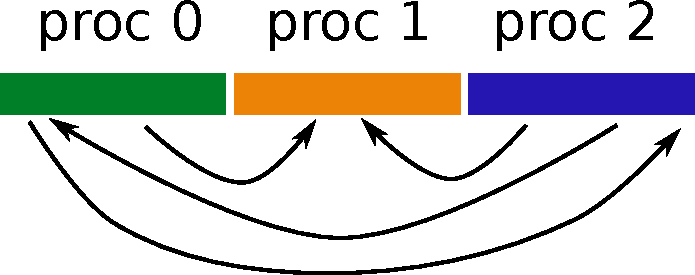
\includegraphics[width=0.75\textwidth]{figures/vectors-scatter} \\[1em]
\begin{lstlisting}
  // y[iy[i]] = x[ix[i]]
  VecScatterCreate(...);
  VecScatterBegin(...);
  VecScatterEnd(...);
\end{lstlisting}
   \end{center}
 \end{block}

\end{frame}

%%%%%%%%%% 


\begin{frame}[fragile]{PETSc Vectors}

 \begin{block}{Vector Reductions}
   \begin{center}
     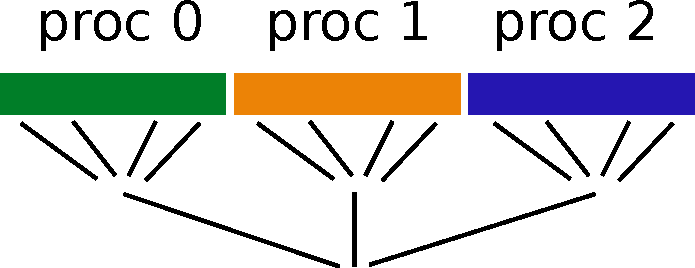
\includegraphics[width=0.75\textwidth]{figures/vectors-reduce} \\[1.2em]
\begin{lstlisting}
  VecNorm(...);
  VecDot(...);
  VecMax(...);
  ...
\end{lstlisting}
   \end{center}
 \end{block}

\end{frame}


%%%%%%%%%% 

\begin{frame}[fragile]{PETSc Vectors}

 \begin{block}{Local (Sequential) Operations}
  \begin{itemize}
   \item Executed by an arbitrary subset of MPI ranks
   \item Usually involve \lstinline|VecGetArray()/VecRestoreArray()|
  \end{itemize}
 \end{block}

 %\pause
 
 \begin{block}{Collective Operations}
  \begin{itemize}
   \item Must be executed by all processes in the MPI communicator
   \item Involve MPI operations (scatter, gather, reduce, etc.)
  \end{itemize}
 \end{block}

\end{frame}


%
% Matrices (preparing for Linear Solvers)
%


\begin{frame}[fragile]{PETSc Application Integration}

\begin{block}{Sparse Matrices}
\begin{itemize}
  \item \textbf{The} important data type when solving PDEs
  \item Two main phases: 
    \begin{itemize}
     \item Filling with entries (assembly)
     \item Application of its action (e.g.~SpMV)
    \end{itemize}
\end{itemize}
\end{block}
\begin{center}
%\includegraphics[width=2in]{figures/Mat/serialSparseMatrix_bcsstk32}
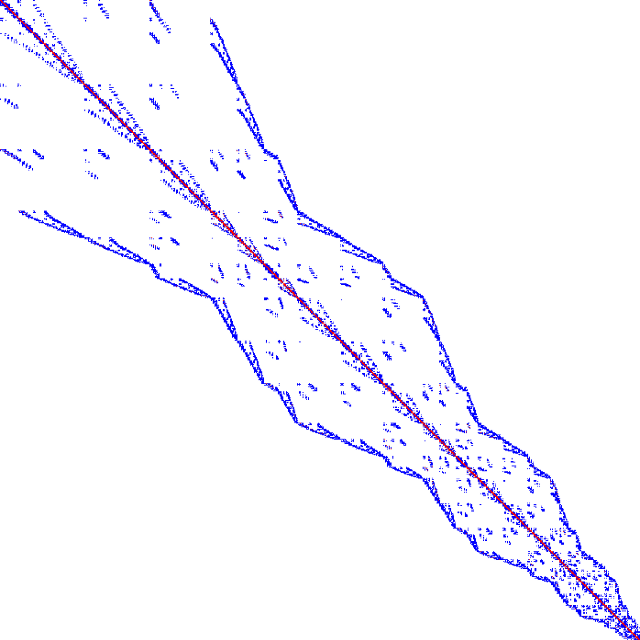
\includegraphics[width=.5\textwidth]{figures/EllipRCMSquare}
\end{center}
\end{frame}



\begin{frame}[fragile]{Matrix Memory Preallocation}
 \begin{block}{PETSc sparse matrices are dynamic data structures}
  \begin{itemize} \vspace*{-0.2cm}
    \item can add additional nonzeros freely
  \end{itemize}
 \end{block}  \vspace*{-0.2cm}

 %\pause
 \begin{block}{Dynamically adding many nonzeros}
  \begin{itemize} \vspace*{-0.2cm}
    \item requires additional memory allocations
    \item requires copies
    \item can kill performance
  \end{itemize}
 \end{block} \vspace*{-0.2cm}

 %\pause
 \begin{block}{Memory preallocation provides}
  \begin{itemize} \vspace*{-0.2cm}
    \item the freedom of dynamic data structures
    \item good performance
  \end{itemize}
 \end{block} \vspace*{-0.2cm}

 %\pause
 \begin{block}{Easiest solution is to replicate the assembly code}
  \begin{itemize} \vspace*{-0.2cm}
    \item Remove computation, but preserve the indexing code
    \item Store set of columns for each row
  \end{itemize}
 \end{block} \vspace*{-0.2cm}

 %\pause
 \begin{block}{Call preallocation routines for all datatypes}
  \begin{itemize} \vspace*{-0.2cm}
    \item \lstinline|MatSeqAIJSetPreallocation()|
    \item \lstinline|MatMPIBAIJSetPreallocation()|
    \item Only the relevant data will be used
  \end{itemize}
\end{block}
\end{frame}




\begin{frame}[fragile]{PETSc Application Integration}

\begin{block}{Sequential Sparse Matrices}
\lstinline|MatSeqAIJSetPreallocation(Mat A, int nz, int nnz[])|
\hbox{\qquad
\vbox{
\begin{itemize}
  \item[nz:] expected number of nonzeros in any row
  \item[nnz(i):] expected number of nonzeros in row i
\end{itemize}
}
}
\end{block}
\begin{center}
%\includegraphics[width=2in]{figures/Mat/serialSparseMatrix_bcsstk32}
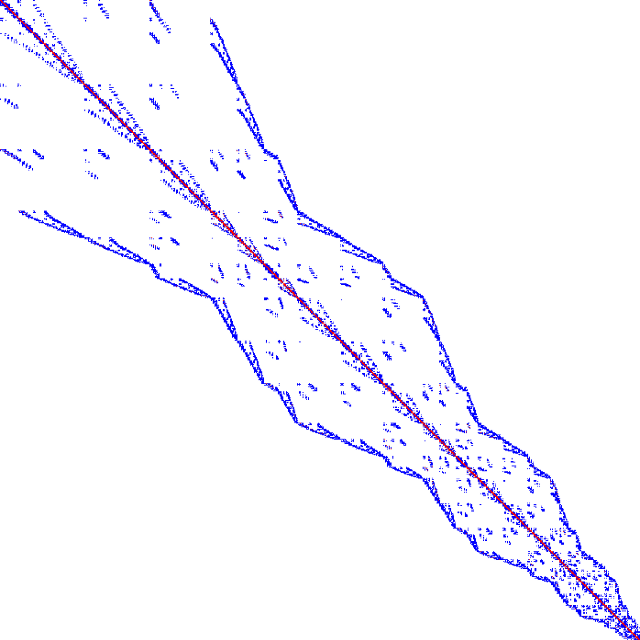
\includegraphics[width=.5\textwidth]{figures/EllipRCMSquare}
\end{center}
\end{frame}

\begin{frame}[fragile]{PETSc Application Integration}

\begin{block}{Parallel Sparse Matrix}
\begin{itemize}
  \item Each process locally owns a submatrix of contiguous global rows
  \item Each submatrix consists of diagonal and off-diagonal parts
\end{itemize}

\begin{center}
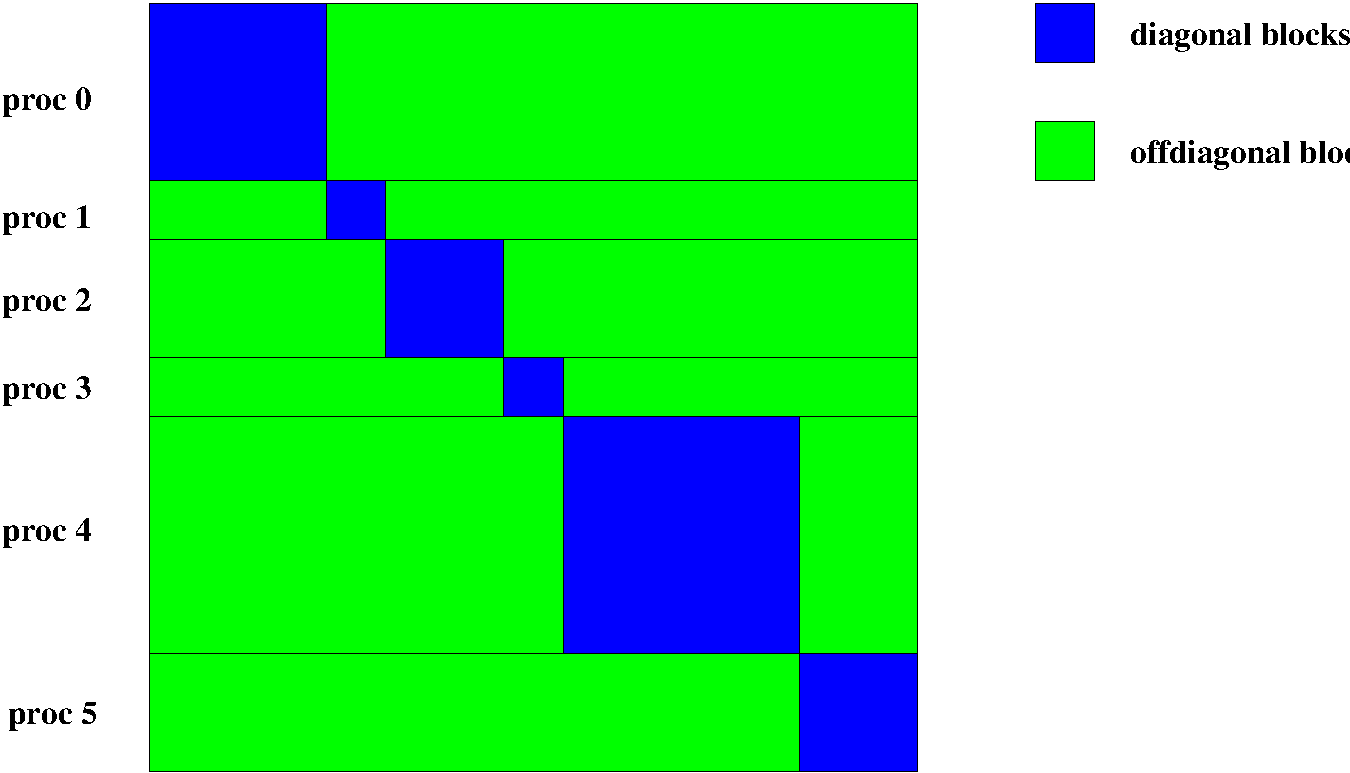
\includegraphics[width=3.in]{figures/Mat/parallelSparseMatrix}
\end{center}

\begin{itemize}
  \item \lstinline|MatGetOwnershipRange(Mat A,int *start,int *end)|
  \begin{itemize}
    \item \lstinline|start|: first locally owned row of global matrix
    \item \lstinline|end-1|: last locally owned row of global matrix
  \end{itemize}
\end{itemize}
\end{block}
\end{frame}


\begin{frame}[fragile]{PETSc Application Integration}

\begin{center}
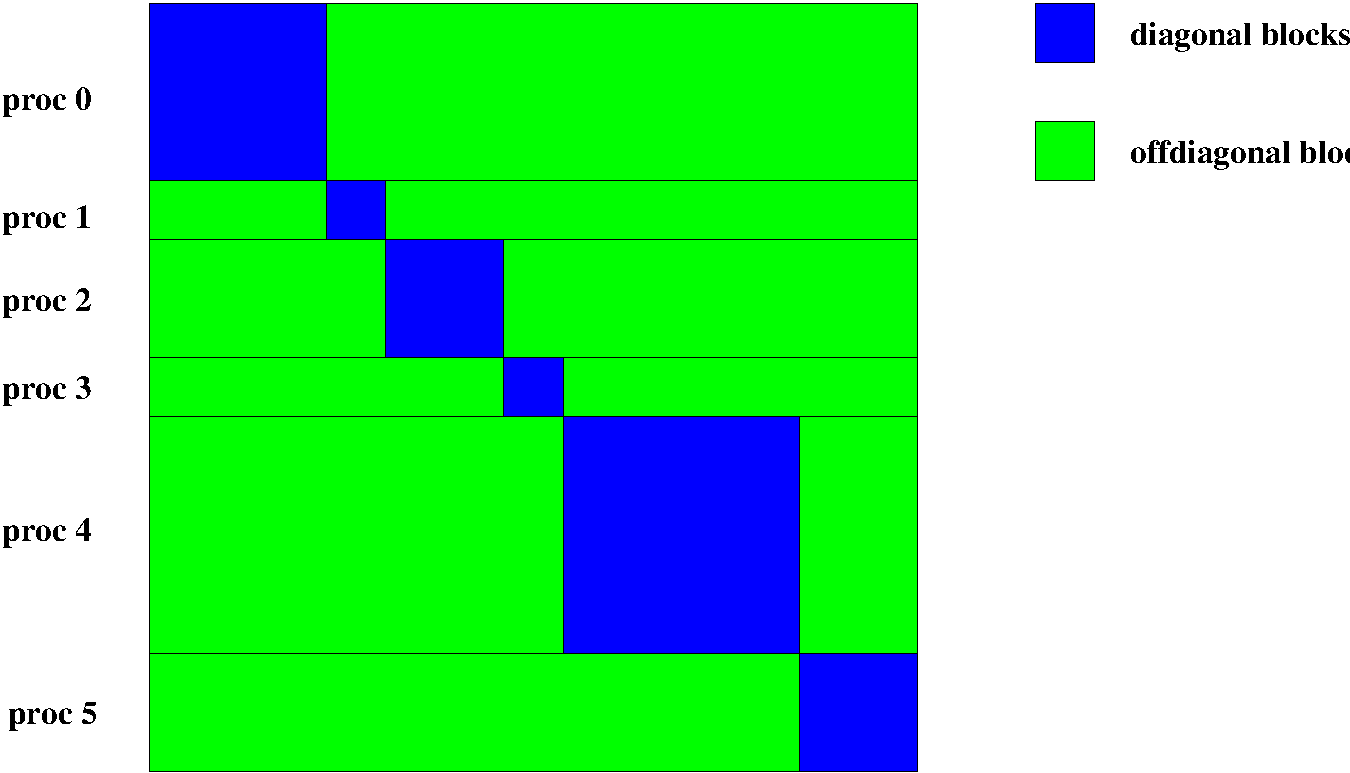
\includegraphics[width=3.in]{figures/Mat/parallelSparseMatrix}
\end{center}

\begin{center}
\begin{tabular}{cc}
\begin{tabular}{c}
\begin{tabular}{|ccc|cc|}
\hline
\multicolumn{3}{|c|}{Proc 2} & \multicolumn{2}{c|}{Proc 3} \\
\hline
25 & 26 & 27 & 28 & 29 \\
20 & 21 & 22 & 23 & 24 \\
15 & 16 & 17 & 18 & 19 \\
\hline
10 & 11 & 12 & 13 & 14 \\
 5 &  6 &  7 &  8 &  9 \\
 0 &  1 &  2 &  3 &  4 \\
\hline
\multicolumn{3}{|c|}{Proc 0} & \multicolumn{2}{c|}{Proc 1} \\
\hline
\end{tabular} \\
Natural numbering
\end{tabular}
& 
\begin{tabular}{c}
\begin{tabular}{|ccc|cc|}
\hline
\multicolumn{3}{|c|}{Proc 2} & \multicolumn{2}{c|}{Proc 3} \\
\hline
21 & 22 & 23 & 28 & 29 \\
18 & 19 & 20 & 26 & 27 \\
15 & 16 & 17 & 24 & 25 \\
\hline
 6 &  7 &  8 & 13 & 14 \\
 3 &  4 &  5 & 11 & 12 \\
 0 &  1 &  2 &  9 & 10 \\
\hline
\multicolumn{3}{|c|}{Proc 0} & \multicolumn{2}{c|}{Proc 1} \\
\hline
\end{tabular}\\
PETSc numbering
\end{tabular}
\end{tabular}
\end{center}

\end{frame}








\begin{frame}[fragile]{PETSc Application Integration}

\begin{block}{Parallel Sparse Matrix}
\vspace{0.5cm}
\hbox{ \quad \vbox{
\begin{lstlisting}
 MatMPIAIJSetPreallocation(Mat A, int dnz, int dnnz[],
                                  int onz, int onnz[]
\end{lstlisting}

\begin{itemize}
  \item[dnz:] expected number of nonzeros in any row in the diagonal block
  \item[dnnz(i):] expected number of nonzeros in row i in the diagonal block
  \item[onz:] expected number of nonzeros in any row in the offdiagonal portion
  \item[onnz(i):] expected number of nonzeros in row i in the offdiagonal portion
\end{itemize}
}}
\end{block}
\end{frame}

\begin{frame}[fragile]{PETSc Application Integration}

\begin{block}{Verifying Preallocation}
\begin{itemize}
  \item Use runtime options 
    \begin{itemize}
      \item \lstinline|-mat_new_nonzero_location_err| 
      \item \lstinline|-mat_new_nonzero_allocation_err|
    \end{itemize}
    
  \item Use runtime option
    \begin{itemize} \item \lstinline|-info| \end{itemize}
  \item Output: \\
\end{itemize}

\end{block}
\begin{lstlisting}[basicstyle=\scriptsize]
[proc #] Matrix size: %d X %d; storage space: %d unneeded, %d used
[proc #] Number of mallocs during MatSetValues( )  is %d
\end{lstlisting}

\begin{center}
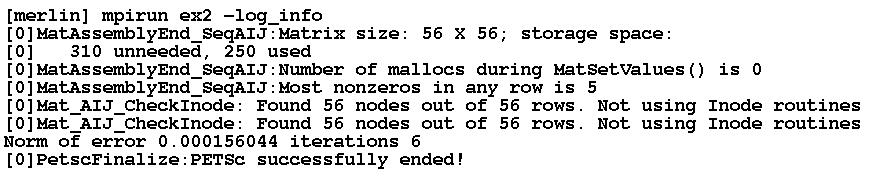
\includegraphics[width=4.in]{figures/logInfoOutput}
\end{center}
\end{frame}

\begin{frame}[fragile]{Block and Symmetric Formats}
  \begin{block}{BAIJ}
    \begin{itemize}
    \item Like AIJ, but uses static block size
    \item Preallocation is like AIJ, but just one index per block
    \end{itemize}
  \end{block}
  
  %\pause
  \begin{block}{SBAIJ}
    \begin{itemize}
    \item Only stores upper triangular part
    \item Preallocation needs number of nonzeros in upper triangular \\
      parts of on- and off-diagonal blocks
    \end{itemize}
  \end{block}
    
  %\pause
  \begin{block}{MatSetValuesBlocked()}
    \begin{itemize}
    \item Better performance with blocked formats
    \item Also works with scalar formats, if \lstinline|MatSetBlockSize()| was called
    \item Variants \lstinline|MatSetValuesBlockedLocal()|, \lstinline|MatSetValuesBlockedStencil()|
    \item Change matrix format at runtime, don't need to touch assembly code
    \end{itemize}
  \end{block}
\end{frame}

\begin{frame}[fragile]{One Way to Set the Elements of a Matrix}

\begin{block}{Simple 3-point stencil for 1D Laplacian}

\begin{lstlisting}
v[0] = -1.0; v[1] = 2.0; v[2] = -1.0;
if (rank == 0) {
  for(row = 0;  row < N; row++) {
    cols[0] = row-1; cols[1] = row; cols[2] = row+1;
    if (row == 0) {
      MatSetValues(A,1,&row,2,&cols[1],&v[1],
                   INSERT_VALUES);
    } else if (row == N-1) {
      MatSetValues(A,1,&row,2,cols,v,INSERT_VALUES);
    } else {
      MatSetValues(A,1,&row,3,cols,v,INSERT_VALUES);
    }
  }
}
MatAssemblyBegin(A,MAT_FINAL_ASSEMBLY);
MatAssemblyEnd(A,MAT_FINAL_ASSEMBLY);
\end{lstlisting}
\end{block}


\end{frame}

\begin{frame}[fragile]{A Better Way to Set the Elements of a Matrix}

\begin{block}{A More Efficient Way}
\small
\begin{lstlisting}
v[0] = -1.0; v[1] = 2.0; v[2] = -1.0;
for(row = start;  row < end; row++) {
  cols[0] = row-1; cols[1] = row; cols[2] = row+1;
  if (row == 0) {
    MatSetValues(A,1,&row,2,&cols[1],&v[1],
                 INSERT_VALUES);
  } else if (row == N-1) {
    MatSetValues(A,1,&row,2,cols,v,INSERT_VALUES);
  } else {
    MatSetValues(A,1,&row,3,cols,v,INSERT_VALUES);
  }
}
MatAssemblyBegin(A, MAT_FINAL_ASSEMBLY);
MatAssemblyEnd(A, MAT_FINAL_ASSEMBLY);
\end{lstlisting}
\end{block}

\begin{block}{Advantages}
 \begin{itemize}
  \item All ranks busy: Scalable!
  \item Amount of code essentially unchanged
 \end{itemize}

\end{block}


\end{frame}



\begin{frame}{Matrices}
  \begin{definition}<1->[Matrix]
    A \alert{matrix} is a linear transformation between finite dimensional vector spaces.
  \end{definition}
  \begin{definition}<1->[Forming a matrix]
    \alert{Forming} or \alert{assembling} a matrix means defining it's action in terms of entries (usually stored in a sparse format).
  \end{definition}
\end{frame}


% Sparse Matrix formats (include benchmark from manual or Jed)
% Matrices in parallel
% Matrix preallocation

\begin{frame}{Matrices}
\begin{block}{Important Matrices}
  \begin{enumerate}
  \item Sparse (e.g.~discretization of a PDE operator)
  \item \alert<2,4>{Inverse of \emph{anything} interesting $B = A^{-1}$}
  \item \alert<4>{Jacobian of a nonlinear function $J y = \lim_{\epsilon \to 0} \frac{F(x + \epsilon y) - F(x)}{\epsilon}$}
  \item \alert<2,4>{Fourier transform $\mathcal{F},\mathcal{F}^{-1}$}
  \item \alert<2,4>{Other fast transforms, e.g. Fast Multipole Method}
  \item \alert<2,4>{Low rank correction $B = A + u v^T$}
  \item \alert<2,4>{Schur complement $S = D - C A^{-1} B$}
  \item \alert<3,4>{Tensor product $A = \sum_e A_x^e \otimes A_y^e \otimes A_z^e$}
  \item \alert<3,4>{Linearization of a few steps of an explicit integrator}
  \end{enumerate}
  \begin{columns}\begin{column}{0.2\textwidth}\end{column}\begin{column}{0.8\textwidth}
  \begin{itemize}
  \item<only@2> These matrices are \alert<2>{dense}.  Never form them.
  \item<only@3>{These are \alert<3>{not very sparse}.}
    Don't form them.
  \item<only@4> {None of these matrices ``have entries''}
  \end{itemize}
\end{column}
\end{columns}
\end{block}
\end{frame}


% \begin{frame}{PETSc}
%    \begin{center} \Large \textbf{What can we do with a matrix \\ which does not have entries?} \\[2em]
%       \visible<2>{\includegraphics[width=0.4\textwidth]{figures/coffee} }
%    \end{center}
% \end{frame}

% 41 distinct slides here




%
% Linear Solvers
%

% Condition number!
\section{Iterative Solvers}
\begin{frame}{PETSc}
   \begin{center} \Large \textbf{Iterative Solvers} \end{center}
\end{frame}

\begin{frame}{Matrices}

\begin{center}
 \em What can we do with a matrix that doesn't have entries?
\end{center}

 %\pause

  \begin{block}{Krylov solvers for $A x = b$}
    \begin{itemize}
    \item Krylov subspace: $\{b, Ab, A^2b, A^3b, \dotsc\}$
    \item Convergence rate depends on the spectral properties of the matrix
      %\begin{itemize}
      %\item Existance of small polynomials $p_n(A) < \epsilon$ where $p_n(0) = 1$.
      %\item condition number $\kappa(A) = \Vert A \Vert \Vert A^{-1} \Vert = \sigma_{\text{max}}/\sigma_{\text{min}}$
      %\item distribution of singular values, spectrum $\Lambda$, pseudospectrum $\Lambda_\epsilon$
%      \item $\epsilon$-pseudospectrum $\Lambda_\epsilon$, spectrum of $A + E$ where $\norm{E} < \epsilon$
      %\end{itemize}
    \item For any popular Krylov method $\mathcal{K}$, there is a matrix
      of size $m$, such that $\mathcal{K}$ outperforms all other methods
      by a factor at least $\mathcal{O}(\sqrt{m})$~[Nachtigal et. al., 1992]%\cite{nachtigal1992fnm}
    \end{itemize}
  \end{block}
  
%\pause

  \begin{block}{Typically...}
    \begin{itemize}
    \item The action $y \gets A x$ can be computed in $\mathcal{O}(m)$
    \item Aside from matrix multiply, the $n^{\text{th}}$ iteration requires at most $\mathcal{O}(mn)$
    \end{itemize}
  \end{block}
\end{frame}


% Dense solvers (reiterate MAGMA-stuff from Day 1)
% Direct solvers (Sparse Gauss, Dissection, etc.)
% Conjugate Gradients
% BiCGStab
\begin{frame}{GMRES}

\begin{block}{Brute force minimization of residual in $\{b,Ab,A^2b,\dotsc\}$}
  \begin{enumerate}
  \item Use Arnoldi to orthogonalize the $n$th subspace, producing
    \[ A Q_n = Q_{n+1} H_n \]
  \item Minimize residual in this space by solving the overdetermined system
    \[ H_n y_n = e_1^{(n+1)} \]
    using $QR$-decomposition, updated cheaply at each iteration.
  \end{enumerate}
\end{block}

%\pause
\begin{block}{Properties}
  \begin{itemize}
  \item Converges in $n$ steps for all right hand sides if there exists a polynomial of degree $n$
    such that $\Vert p_n(A) \Vert < \textit{tol}$ and $p_n(0)=1$.
  \item Residual is monotonically decreasing, robust in practice
  \item Restarted variants are used to bound memory requirements
  \end{itemize}
\end{block}
\end{frame}


\begin{frame}[fragile]{PETSc Solvers}

\begin{block}{Linear Solvers - Krylov Methods}
 \begin{itemize}
  \item Using PETSc linear algebra, just add:
  \begin{lstlisting}[basicstyle=\footnotesize\ttfamily]
KSPSetOperators(KSP ksp, Mat A, Mat M, MatStructure flag)
KSPSolve(KSP ksp, Vec b, Vec x)
  \end{lstlisting}

  \item Can access subobjects
  \begin{lstlisting}[basicstyle=\footnotesize\ttfamily]
KSPGetPC(KSP ksp, PC *pc)
  \end{lstlisting}

  \item Preconditioners must obey PETSc interface
  \begin{itemize}
    \item Basically just the KSP interface
  \end{itemize}

  \item Can change solver dynamically from the command line, \lstinline|-ksp_type|
\end{itemize}
\end{block}

\end{frame}


\begin{frame}{Linear solvers in PETSc KSP}
 \begin{block}{Linear solvers in PETSc KSP (Excerpt)}
  \begin{itemize}
  \item Richardson
  \item Chebychev
  \item Conjugate Gradient
  \item BiConjugate Gradient
  \item Generalized Minimum Residual Variants
  \item Transpose-Free Quasi-Minimum Residual
  \item Least Squares Method
  \item Conjugate Residual
  \end{itemize}
 \end{block}
\end{frame}





%
%%%%% Preconditioners
% 

\section{Preconditioners}
\begin{frame}{PETSc}
   \begin{center} \Large \textbf{Preconditioners} \end{center}
\end{frame}

\subsection{Preconditioning}
\begin{frame}{Preconditioning}
  \begin{block}{Idea: improve the conditioning of the Krylov operator}
    \begin{itemize}
    \item Left preconditioning
      \vspace{-1em}
      \begin{gather*}
        (P^{-1} A) x = P^{-1} b \\
        \{ P^{-1} b, (P^{-1}A) P^{-1} b, (P^{-1}A)^2 P^{-1} b, \dotsc \}
      \end{gather*}
    \item Right preconditioning
      \vspace{-1em}
      \begin{gather*}
        (A P^{-1}) P x = b \\
        \{ b, (P^{-1}A)b, (P^{-1}A)^2b, \dotsc \}
      \end{gather*}
    \item The product $P^{-1}A$ or $A P^{-1}$ is \emph{not} formed.
    \end{itemize}
  \end{block}
  %\begin{definition}[Preconditioner]
      A \emph{preconditioner} $\mathcal{P}$ is a method for constructing a
matrix (just a linear function, not assembled!)  $P^{-1} = \mathcal{P}(A,A_p)$
using a matrix $A$ and extra information $A_p$, such that the spectrum
of $P^{-1}A$ (or $A P^{-1}$) is well-behaved.
   % \end{definition}
\end{frame}

\begin{frame}{Preconditioning}
  \begin{definition}[Preconditioner]
      A \emph{preconditioner} $\mathcal{P}$ is a method for constructing a matrix
      $P^{-1} = \mathcal{P}(A,A_p)$ using a matrix $A$ and extra information $A_p$, such that
      the spectrum of $P^{-1}A$ (or $A P^{-1}$) is well-behaved.
    \end{definition}
    \begin{itemize}
    \item $P^{-1}$ is dense, $P$ is often not available and is not needed
    \item $A$ is rarely used by $\mathcal{P}$, but $A_p = A$ is common
    \item $A_p$ is often a sparse matrix, the ``preconditioning matrix''
    \item Matrix-based: Jacobi, Gauss-Seidel, SOR, ILU(k), LU
    \item Parallel: Block-Jacobi, Schwarz, Multigrid, FETI-DP, BDDC
    \item Indefinite: Schur-complement, Domain Decomposition, Multigrid
    \end{itemize}
\end{frame}


\begin{frame}{Questions to ask when you see a matrix}
  \begin{enumerate}
  \item What do you want to do with it?
    \begin{itemize}
    \item Multiply with a vector
    \item Solve linear systems or eigen-problems
    \end{itemize}
  \item How is the conditioning/spectrum?
    \begin{itemize}
    \item distinct/clustered eigen/singular values?
    \item symmetric positive definite ($\sigma(A) \subset \mathbb{R}^+$)?
    \item nonsymmetric definite ($\sigma(A) \subset \{z \in \mathbb{C} : \mathrm{Re} [z] > 0 \}$)?
    \item indefinite?
    \end{itemize}
  \item How dense is it?
    \begin{itemize}
    \item block/banded diagonal?
    \item sparse unstructured?
    \item denser than we'd like?
    \end{itemize}
  \item Is there a better way to compute $Ax$?
  \item Is there a different matrix with similar spectrum, but nicer properties?
  \item \alert<2>{How can we precondition $A$?}
  \end{enumerate}
\end{frame}

\begin{frame}{Relaxation}
  Split into lower, diagonal, upper parts: \alert{$ A = L + D + U $}
  \begin{block}{Jacobi}
    Cheapest preconditioner: $P^{-1} = D^{-1}$
  \end{block}
  \begin{block}{Successive over-relaxation (SOR)}
    \begin{gather*}
      \left(L + \frac 1 \omega D\right) x_{n+1} = \left[\left(\frac
          1\omega-1\right)D - U\right] x_n + \omega b \\
      P^{-1} = \text{$k$ iterations starting with $x_0=0$}
    \end{gather*}
    \begin{itemize}
    \item Implemented as a sweep
    \item $\omega = 1$ corresponds to Gauss-Seidel
    \item Very effective at removing high-frequency components of residual
    \end{itemize}
  \end{block}
\end{frame}

\begin{frame}[shrink=5]{Factorization}
  \begin{block}{Two phases}
  \begin{itemize}
  \item symbolic factorization: find where fill occurs, only uses sparsity pattern
  \item numeric factorization: compute factors
  \end{itemize}
  \end{block}
  
  
  \begin{block}{LU decomposition}
    \begin{itemize}
    \item Ultimate preconditioner
    \item Expensive, for $m\times m$ sparse matrix with bandwidth $b$, traditionally requires $\mathcal{O}(mb^2)$ time and $\mathcal{O}(mb)$ space.
      \begin{itemize}
      \item Bandwidth scales as $m^{\frac{d-1}{d}}$ in $d$-dimensions
      \item Optimal in 2D: $\mathcal{O}(m \cdot \log m)$ space, $\mathcal{O}(m^{3/2})$ time
      \item Optimal in 3D: $\mathcal{O}(m^{4/3})$ space, $\mathcal{O}(m^2)$ time
      \end{itemize}
    \item Symbolic factorization is problematic in parallel
    \end{itemize}
  \end{block}
  \begin{block}{Incomplete LU}
    \begin{itemize}
    \item Allow a limited number of levels of fill:
      ILU($k$)
    \item Only allow fill for entries that exceed threshold: ILUT
    \item Usually poor scaling in parallel
    \item No guarantees
    \end{itemize}
  \end{block}
\end{frame}

\begin{frame}{1-level Domain decomposition}
  Domain size $L$, subdomain size $H$, element size $h$
  \begin{block}{Overlapping/Schwarz}
    \begin{itemize}\item Solve Dirichlet problems on overlapping
      subdomains
    \item No overlap: $\textit{its} \in \mathcal{O}\big( \frac{L}{\sqrt{Hh}} \big)$
    \item Overlap $\delta$: $\textit{its} \in \big( \frac L {\sqrt{H\delta}} \big)$
    \end{itemize}
  \end{block}
  \begin{block}{Neumann-Neumann}
    \begin{itemize}
    \item Solve Neumann problems on non-overlapping subdomains
    \item $\textit{its} \in \mathcal{O}\big( \frac{L}{H}(1+\log\frac H h) \big)$
    \item Tricky null space issues (floating subdomains)
    \item Need subdomain matrices, net globally assembled matrix.
    \end{itemize}
  \end{block}
  \begin{itemize}
  \item Multilevel variants knock off the leading $\frac L H$
  \item Both overlapping and nonoverlapping with this bound
  \end{itemize}
  % \begin{block}{BDDC and FETI-DP}
  %   \begin{itemize}
  %   \item Neumann problems on subdomains with
  %     coarse grid correction
  %   \item $\textit{its} \in \bigO\big(1 + \log\frac H h \big)$
  %   \end{itemize}
  %   \includegraphics[width=0.7\textwidth]{bddc}
  % \end{block}
\end{frame}

\begin{frame}[shrink=5]{Multigrid}
  \begin{block}{Hierarchy: Interpolation and restriction operators}
    \begin{equation*}
    \mathcal{I}^\uparrow : X_{\text{coarse}} \to X_{\text{fine}} \qquad
    \mathcal{I}^\downarrow :  X_{\text{fine}} \to X_{\text{coarse}}
  \end{equation*}
  \end{block}
  \begin{itemize}
  \item Geometric: define problem on multiple levels, use grid to compute hierarchy
  \item Algebraic: define problem only on finest level, use matrix structure to build hierarchy
  \end{itemize}
  \begin{block}{Galerkin approximation}
    Assemble this matrix: $A_{\text{coarse}} = \mathcal{I}^\downarrow A_{\text{fine}} \mathcal{I}^\uparrow$
  \end{block}
  \begin{block}{Application of multigrid preconditioner ($V$-cycle)}
    \begin{itemize}
    \item Apply pre-smoother on fine level (any preconditioner)
    \item Restrict residual to coarse level with $\mathcal{I}^\downarrow$
    \item Solve on coarse level $A_{\text{coarse}} x = r$
    \item Interpolate result back to fine level with $\mathcal{I}^\uparrow$
    \item Apply post-smoother on fine level (any preconditioner)
    \end{itemize}
  \end{block}
\end{frame}

\begin{frame}{Multigrid convergence properties}
  \begin{itemize}
  \item Textbook: $P^{-1}A$ is spectrally equivalent to identity
    \begin{itemize}
    \item Constant number of iterations to converge up to discretization error
    \end{itemize}
  \item Most theory applies to SPD systems
    \begin{itemize}
    \item variable coefficients (e.g.~discontinuous): low energy interpolants
    \item mesh- and/or physics-induced anisotropy: semi-coarsening/line smoothers
    \item complex geometry: difficult to have meaningful coarse levels
    \end{itemize}
  \item Deeper algorithmic difficulties
    \begin{itemize}
    \item nonsymmetric (e.g.~advection, shallow water, Euler) \\
    \item indefinite (e.g.~incompressible flow, Helmholtz)
    \end{itemize}
  \item Performance considerations
    \begin{itemize}
    \item Aggressive coarsening is critical in parallel
    \item Most theory uses SOR smoothers, ILU often more robust
    \item Coarsest level usually solved semi-redundantly with direct solver
    \end{itemize}
  \item Multilevel Schwarz is essentially the same with different language
    \begin{itemize}
    \item assume strong smoothers, emphasize aggressive coarsening
    \end{itemize}
  \end{itemize}
\end{frame}


% Explain various preconditioners here:
%   - Jacobi, Block-Jacobi
%   - SPAI
%   - ICC/ILU (include symbolic stage)
%   - Multigrid (geometric, algebraic)
%\input{slides/PreconditioningSamples.tex}



% Intermediate summary: Preconditioners for single quantity


\begin{frame}{Splitting for Multiphysics}
  \begin{equation*}
    \begin{bmatrix}
      A & B \\ C & D
    \end{bmatrix}
    \begin{bmatrix}
      x \\ y
    \end{bmatrix}
    =
    \begin{bmatrix}
      f \\ g
    \end{bmatrix}
  \end{equation*}
  \begin{itemize}\item Relaxation: \lstinline|-pc_fieldsplit_type| \newline
    \lstinline| [additive,multiplicative,symmetric_multiplicative]|
    \begin{equation*}
      \begin{bmatrix}
        A & \\  & D
      \end{bmatrix}^{-1} \qquad 
      \begin{bmatrix}
        A & \\ C & D
      \end{bmatrix}^{-1} \qquad
      \begin{bmatrix}
        A & \\  & \mathbf{1}
      \end{bmatrix}^{-1}
      \left(
        \mathbf{1} -
        \begin{bmatrix}
          A & B \\ & \mathbf{1}
        \end{bmatrix}
        \begin{bmatrix}
          A & \\ C & D
        \end{bmatrix}^{-1}
      \right)
    \end{equation*}
    \begin{itemize}
    \item Gauss-Seidel inspired, works when fields are loosely coupled
    \end{itemize}
  \item Factorization: \lstinline|-pc_fieldsplit_type schur|
    \begin{align*}
      \begin{bmatrix}
        A & B \\ & S
      \end{bmatrix}^{-1}
      \begin{bmatrix}
        \mathbf{1} & \\ CA^{-1} & \mathbf{1}
      \end{bmatrix}^{-1}, \qquad
      S = D - C A^{-1} B
    \end{align*}
    \begin{itemize}
    \item robust (exact factorization), can often drop lower block
    \item how to precondition $S$ which is usually dense?
      \begin{itemize}
      \item interpret as differential operators, use approximate commutators
      \end{itemize}
    \end{itemize}
  \end{itemize}
\end{frame}

% Compose preconditioners for multiple fields (Fun with Matt)


%%%% Conclusion


\section{Conclusion}
\begin{frame}{End of Lecture}
 
 \begin{block}{Distributed Systems}
  \begin{itemize}
   \item Mind data partitioning
   \item Asymptotics of solvers important
   \item Reuse existing packages!
  \end{itemize}
 \end{block}

 \pause
 \begin{block}{General Recommendations}
  \begin{itemize}
   \item Consult literature for preconditioners
   \item Performance modeling is very handy
   \item Your time is more valuable than computing time!
  \end{itemize}
 \end{block}

\end{frame}
